\documentclass[12pt]{article}
\usepackage[paper=a4paper,left=25mm,right=25mm,top=30mm,bottom =30mm]{geometry}
\usepackage[utf8]{inputenc}
\usepackage[T1]{fontenc}
\usepackage{stmaryrd}
\usepackage{extarrows}
%\usepackage{ccc-arrows}
\usepackage{setspace}
\usepackage{mathrsfs}
\usepackage{mathtools}
\usepackage[ngerman]{babel}
\usepackage{amssymb}
\usepackage{amsmath}
\usepackage{fancyhdr}
\usepackage[dvips,unicode,colorlinks,linkcolor=black]{hyperref} 
\usepackage{graphicx}
\usepackage{float}




\pagestyle{fancy}
\lfoot{}
\rfoot{Paul Kremser, Tobias Grussenmeyer}
\cfoot{\thepage}
\fancyhead[L]{FPI Versuch: SQUID}
\renewcommand{\headrulewidth}{0.6pt}
\renewcommand{\footrulewidth}{0.6pt}
\setlength{\headheight}{16pt}
\setlength{\parindent}{0pt}
% Für die Wahl der Schriftart
\newcommand{\changefont}[3]{
\fontfamily{#1} \fontseries{#2} \fontshape{#3} \selectfont}

\begin{document}
% keine Hurenkinder und Schusterjungen
\clubpenalty = 10000
\widowpenalty = 10000 
\displaywidowpenalty = 10000

\onehalfspacing
% Schriftart
\changefont{ptm}{m}{n} 

\begin{titlepage}
\author{Paul Kremser, Tobias Grussenmeyer}
\title{Versuch: SQUID}
\date{Versuchsdurchführung: 22. Oktober 2009} 
\maketitle
\thispagestyle{empty}
\end{titlepage}


\tableofcontents
\thispagestyle{empty}
\newpage
\pagenumbering{arabic}
\section{Überblick}
In diesem Versuch soll mittels eines \textit{SQUID} das Magnetfeld verschiedener Proben sowie einer Stromdurchflossenen Leiterschleife gemessen und deren Dipolmoment bestimmt werden. Ein SQUID (\textbf{S}uper\-conducting \textbf{Qu}antum \textbf{I}nterference \textbf{D}evice) ist ein sehr kleiner, höchst empfindlicher Magnetfelddetektor, mit dem sich äußerst geringe Magnetfeldschwankungen registrieren lassen. Da die Nachweisgenauigkeit nur durch Quanteneffekte begrenzt ist, wird die Messgenauigkeit von keinem anderen Magnetfelddetektor übertroffen. Im wesentlichen besteht ein SQUID nur aus einem supraleitendem Ring der an einer sehr schmalen Stelle durch einen Isolator unterbrochen ist. Mit Hilfe geeigneter Elektronik können so kleinste Flussänderungen im Innern des Rings erkannt werden.


\section{Aufgabenstellung}
\begin{enumerate}
 \item Kalibration das SQUID durch Variation der Einstellungen. Es soll eine möglichst große Amplitude des SQUID-Patterns bei möglichst kleinem Rauschen gefunden werden.
\item Vermessung der Magnetfelder einer rotierender Leiterschleife welche von fünf verschiedenen Stromstärken durchflossen wird.  Bestimmung der Dipolmomente und Vergleich mit berechnetem Wert.
\item Vermessung der Magnetfelder und Dipolmomente verschiedener Proben (Magnetspan, Stabmagnet, Geldstück, SIM-Karte)
\item (optional) polare Darstellung der Stärke des Magnetfeldes in Abhängigkeit des Drehwinkels
\end{enumerate}
\newpage

\section{Theoretische Grundlagen}
\subsection{Supraleitung}
Bei der normalen elektrischen Leitung entsteht der elektrische Widerstand durch Wechselwirkungen der Elektronen mit Gitterfehlern des Kristallgitters und Gitterschwingungen. Darüber hinaus können auch Streuprozesse der Elektronen untereinander eine wichtige Rolle spielen. Vor der  Entdeckung der Supraleitung nahm man an, dass der elektrische Widerstand bei sinkender Temperatur asymptotisch gegen einen konstanten Wert (der nun nur noch aus der Wechselwirkung der Elektronen mit den Gitterfehlern resultiert) ginge. Anders als erwartet stellte sich jedoch heraus, dass für einige Stoffe der Wiederstand unterhalb einer kritischen Temperatur schlagartig einen nicht messbaren Wert annimmt. Dieses Phenomen bezeichnet man als Supraleitung. Unter Supraleitung versteht man also elektrische Leitung ohne messbaren Widerstand, man spricht auch von einem Suprastrom. \\
\begin{figure}[H]  %Gotische Kathedrale Kap. 4.1
\begin{minipage}{0.5\linewidth}
\centering
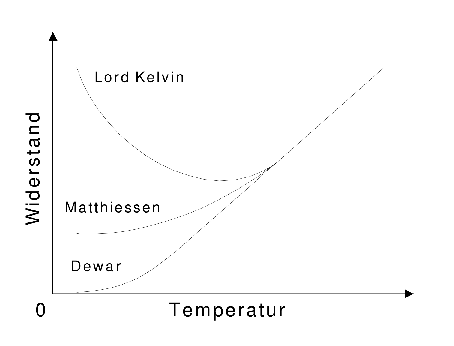
\includegraphics[width=0.9\linewidth]{pictures/wiederstandTemp.eps}
\caption{Elektrischen Widerstandes bei tiefen Temperaturen. Vorstellungen um 1900.}
\end{minipage}
\begin{minipage}{0.5\linewidth}
\centering 
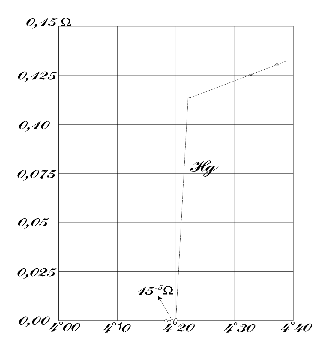
\includegraphics[width=0.9\linewidth]{pictures/HGJump.eps}
\caption{Sprungtemperatur von Quecksilber (Leiden 1911)}
\end{minipage}
\end{figure}

Allgemein wird die Supraleitung durch eine Paarbildung von Elektronen (Cooper-Paare) im Leiter erklärt(siehe hierzu \ref{bcs}).
 Durch die Kopplung der Elektronen im Supraleiter zu Cooper-Paaren wird die Energieabgabe an das Kristallgitter unterdrückt und so der widerstandslose elektrische Stromfluss ermöglicht. \\

Supraleiter sind ideale Diamagneten, im supraleitenden Zustand vermag ein Supraleiter bis zu einer oberen kritischen Grenze ein äußeres Magnetfeld (bis auf eine exponentiell abfallende Eindringtiefe an der Oberfläche, siehe \ref{london}) vollständig aus seinem Inneren zu verdrängen.\\

Es sind zwei Arten von Supraleitern bekannt: Typ-I und Typ-II.

Bei Typ I Supraleitern existiert nur eine obere kritische Grenze des äußeren Magnetfeldes. Unterhalb dieser befindet sich der Supraleiter in der Meißner-Phase, überschreitet das Magnetfeld diese Grenze so bricht die Supraleitung zusammen.\\

Bei Typ II Supraleitern gibt es zwei kritische äußere Magnetfelder, bis zum ersten kritischen Feld verhält sich der Supraleiter wie Typ I, darüber können magnetische Feldlinien in Form so genannter Flussschläuche in das Material eindringen, ehe der supraleitende Zustand bei dem oberen kritischen Magnetfeld vollständig zerstört wird. Der magnetische Fluss in den Flussschläuchen beträgt immer ein ganzzahliges Vielfaches des magnetischen Flussquants (siehe \ref{flussquantisierung}).\\

Bei unserem SQUID handelt es sich um einen Typ II Supraleiter. Beispiele für solche sind die keramischen Hochtemperatursupraleiter. Zwei wichtige Gruppen sind YBaCuO (Yttrium- Barium- Kupferoxide) und BiSrCaCuO (Bismut- Strontium- Kalzium- Kupferoxide). Weiterhin zählen die meisten supraleitenden Legierungen zum Typ II, so die für MR-Magnete verwendeten Niob-Aluminium-Legierungen.

\subsection{BCS-Theorie}
\label{bcs}
Nach der BCS-Thorie sind die Elektronen bei tiefer Temperatur gepaart. Die Kopplung beruht auf einer Wechselwirkung zwischen den Elektronen und dem Kristallgitter. Ein Elektron wechselwirkt mit dem Gitter und deformiert es. Das gestörte Gitter wechselwirkt, seinerseits mit einem anderen Elektron in der Weise, dass zwischen den beiden Elektronen eine Anziehung besteht, die bei niedrigen Temperaturen stärker als die Coulomb-Abstoßung ist. Die beiden Elektronen gehen in einen gebundenen Zustand über und bilden ein so genanntes Cooper-Paar. Die beiden Elektronen in einem Cooper-Paar haben entgegengesetzte Spins, so dass das Cooper-Paar als Ganzes den Spin null hat. Jedes Cooper-Paar verhält sich also wie ein Boson. Bosonen unterliegen nich dem Pauli-Verbot, so dass sich belibig viele Cooper-Paare im gleichen Quantenzustand befinden und die gleiche Energie besitzen können. Im Grundzustand des Supraleiters bei $T = 0K$ sind alle Elektronen in Cooper-Paaren gebunden, und alle Cooper-Paare haben dieselbe Energie. Im supraleitenden Zustand sind die Cooper-Paare stark korreliert und verhalten sich immer alle gleich. Der Stromfluss im Supraleiter wird dabei so realisiert, dass sich alle Elektronen in diesem Kollektiv gemeinsam bewegen. Dagegen kann Energiesissipation, die auf Stößen einzelner Elektronen mit den Gitterionen beruht, nicht stattfinden, es sei denn, die Temperatur ist so hoch, dass die Bindung der Cooper-Paare aufgebrochen wird. \\

\textbf{Ergebnisse der BCS-Theorie:} \\

Die Reichweite $r_0$ bzw. die Ausdehnung der Elektronen-Paarwellenfunktion berechnet sich zu:
\begin{align}
r_0 \propto \frac{\hbar}{\partial p} \propto \frac{\hbar v_F}{\Delta E} \propto \frac{E_F}{k_F \Delta E}
\end{align}

Mit $E_F \approx (10^3 ~\textnormal{bis}~ 10^4) \cdot \Delta E$ und $k_F \approx 10^8~ cm^{-1}$ erhält man für $r_0$ Ergebnisse in der Ordnung von $10^3$ \AA

Dieses Resultat, wenn auch nur abgeschätzt, ist wichtig, denn es impliziert zwei Sachverhalte: Erstens
ist der Bereich der Aufenthaltswahrscheinlichkeiten der beiden Elektronen so groß, dass die Wellenfunk-
tionen der Paare sich mehrfach uberlappen, was zur Bildung eines kohärenten Gesamtzustandes führt.
Zweitens wird dies, siehe unten, zu Tunnelphänomenen durch dünne Schichten führen.
Die kritische Temperatur $T_C$, welche angibt, wann das Material ohne Einfluss eines äußeren Magnetfeldes 
in den supraleitenden Zustand übergeht, berechnet sich zu:
\begin{align}
 T_C = \frac{1,13}{k_B} \hbar \omega e^{-1/D_0 V_0}
\end{align}

$k_B$ steht für die Boltzmann-Konstante, $D_0$ die Zustandsdichte des (noch) normalleitenden Materials und
$V_0$ sowie $\hbar \omega$ sind definiert durch den ursprünglichen Hamiltonoperator. Der Exponent der e-Funktion
liegt etwa in dem Bereich [-2, ... , -10].
Für die Energielücke bei $T = 0 K$ erhält man:
\begin{align}
 \Delta E(0) = 2\hbar\omega e^{-1 / D_0 V_0}
\end{align}

Die Energielücke ist allerdings temperaturabhängig. Sie wird schmaler, wenn sich die Temperatur in
Größenordnung der Sprungtemperatur befindet. Dort verhält sie sich nach
\begin{align}
 \frac{\Delta E(T)}{\Delta E(0)} = 1,74 \sqrt{ 1 - \frac{T}{T_C}}
\end{align}
In ähnlicher Weise ergibt sich das temperaturabhängige Verhalten des kritischen Feldes Hc :
\begin{align}
 \frac{H_C(T)}{H_C} \approx 1 - \left( \frac{T}{T_C} \right)^2
\end{align}

\subsection{Flussquantisierung}
\label{flussquantisierung}

Bei einem SQUID handelt es sich um einen kreisförmigen Supraleiter, der Kreisstrom im Innern lässt sich also als Wegintegral über die Stromdichte $\vec{j}$ berechnen. Da dieser natürlich Null sein muss, folgt
\begin{align}
 \label{kreisstrom} \oint_C \vec j ~ d\vec l = 0
\end{align}

wobei $C$ der Weg entlang des SQUID's ist. Mit dem Stoke'schen Satz folgt das sich der magnetischen Fluss $\Phi_B$ durch den Ring darstellen lässt als das geschlossene Integral über das Vektorfeld $\vec A$:
\begin{align}
 \oint\vec A~d\vec l = \Phi_B
\end{align}

Die Cooper-Paare liegen wie oben beschrieben alle im gleichen Zustand vor, weshalb sie durch eine gemeinsame Wellenfunktion beschrieben werden können. Die Phase $\theta$ dieser Wellenfunktion ist ein eindeutiger Parameter, daher kann sie sich beim Umlauf um den Ring nur um Vielfache von $2\pi$ ändern:
\begin{align}
\label{phase}\oint \vec\nabla \theta d\vec l = \Delta\theta = n~2\pi
\end{align}

Aus Gleichungen \ref{kreisstrom} - \ref{phase} folgt somit eine Quantisierung des magnetischen Flusses in Vielfache von $\Phi_0$, Fluxoide genannt:
\begin{align}
  \left|\Phi_B\right| &= n\frac{\hbar c}{2 e} = n \Phi_0 \\
\notag \\
\notag \textnormal{mit}~~\Phi_0 &= 2,067833667(52)\cdot 10^{-15} ~ Wb \quad \quad (1[Wb] = 1[Tm^2])
\end{align}

\newpage

\subsection{London-Gleichungen}
\label{london}
Die Londongleichungen geben Aufschluss über die Eindringtiefe eines äußeren Magnetfelds in einen Supraleiter.
Hierzu wird angenommen, dass Beschleunigung von Ladungen $e$ nur von einem statischen elektrischen Feld $\vec E$ herrühren:
\begin{align}
 m~\dot{\vec{v}}_e = - e~ \vec E
\end{align}
Dies zusammen mit der Stromdichte $\vec j = n_e e~\vec v_e$, wobei $n_e$ Ladungsdichte, in die beiden Maxwellgleichungen:
\begin{align}
 \vec\nabla \times \vec E = - \frac{1}{c}\frac{\partial\vec B}{\partial t} \textnormal{\quad und \quad} 
 \vec\nabla \times \vec B =  \frac{4~\pi}{c}~\vec j
\end{align}
- durch ableiten der Stromdichte nach der Zeit - eingesetzt, liefert
\begin{align}
 \frac{\partial}{\partial t} \left( \vec\nabla\times\vec j +  \frac{n_e~e^2}{m~c}~\vec B\right) = 0
\end{align}
Dies fordert Zeitliche Invarianz des Ausdrucks in der Klammer, da $\vec B$ im inneren des Supraleiters aber Null ist, folgt dass die Klammer Null sein muss. Somit kommt man auf die London-Gleichung:
\begin{align}
 \vec\nabla\times\vec j = -\frac{n_e~e^2}{m~c}~\vec B
\end{align}
aus der sich die beiden Gleichungen:
\begin{align}
 \nabla^2~\vec B = \frac{4~\pi~n_e~e^2}{m~c^2}~\vec B \textnormal{\quad und \quad} \nabla^2~\vec j = \frac{4~\pi~n_e~e^2}{m~c^2}~\vec j
\end{align}
ableiten lassen. Lösungen für diese sind exponentiell abfallende Funktionen mit einer Reichweite von $\Lambda =\sqrt{\frac{m~c^2}{4~\pi~n_e~e^2}}$. Folglich kann ein äußeres Magnetfeld eine gewisse Länge in einen Supraleiter eindringen. In der vom Magnetfeld durchdrungenen Schicht fliesst ein Abschirmstrom senkrecht zum Magnetfeld.
\newpage

\subsection{Josephson-Effekt}
\label{josephson}

Der Josephson-Effekt besagt, dass Cooper-Paare widerstandsfrei zwischen zwei Supraleitern tunneln, die durch eine dünne, nichtsupraleitende Schicht voneinander getrennt sind. Eine solche Anordnung nennt man \textbf{Josephson-Kontakt}. Der Tunnelstrom tritt auf, ohne dass eine Spannung über dem Kontakt angelegt wird. Der Strom hängt von der Phasendifferenz der Wellenfunktion der Cooper-Paare in den beiden Supraleitern ab. Sei $\phi_1$ die Phase der Wellenfunktion eines Cooper-Paars in dem einen Supraleiter. Dann haben auch alle anderen Cooper-Paare in diesem Supraleiter die Phase $\phi_1$, da sich alle Cooper-Paare in einem Supraleiter kohärent verhalten. Ist $\phi_2$ die Phase der Wellenfunktionen aller Cooper-Paare im zweiten Supraleiter, so beträgt der Strom durch die Übergangsschicht:
\begin{align}
\label{jos-gleichstrom}
 I = I_{max}~sin(\phi_2 - \phi_1)
\end{align}
Darin ist $I_{max}$ der maximale Strom. Dieser ist von der Dicke der Kontaktschicht abhängig. Die Gleichung \ref{jos-gleichstrom} beschreibt die Abhängigkeit die als \textbf{Josephson-Gleichstrom-Effekt} bezeichnet wird.


\subsection{Das SQUID}

Das SQUID kann also kleinste magnetische Flussänderungen in der grössenordnung eines Flussquants registrieren. Es gibt verschiedene technische Umsetzungen, hier im Praktikum  nutzen wir ein sogenanntes RF-SQUID (RF = Radio Frequency),  ein vergleichsweise einfacher und günstiger Aufbau.
\newpage
\subsubsection{Aufbau des RF-SQUID}

Das RF-SQUID besteht im wesentlichen aus einem ringförmigen Hochtemperatursupraleiter, der an einer Stelle durch eine sehr dünne Isolatorschicht unterbrochen ist und einem LC-Schwingkreis. Die Isolatorschicht ist nur wenige nm dick  und erfüllt die Funktion eines Josephson-Kontaktes.

\begin{figure}[H]
\centering
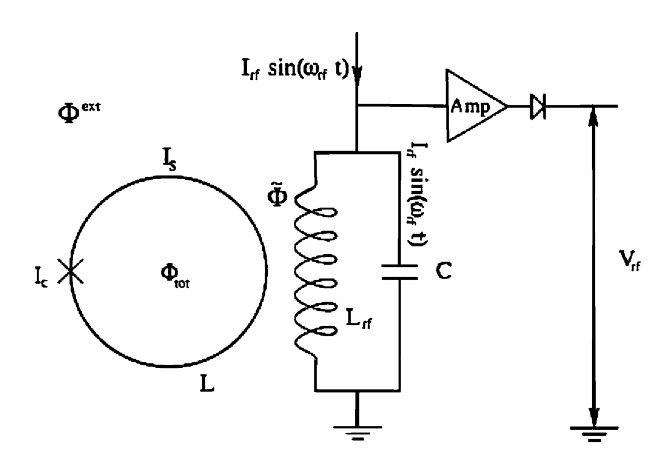
\includegraphics[width=0.9\linewidth]{pictures/rfSQUID.eps}
\caption{Aufbau unseres Radio Frequency SQUID.}
\end{figure}

Die  kritische Temperatur wird durch eintauchen des SQUIDS in Stickstoff erreicht. Der Schwingkreis wird mit einer Frequenz von einigen hundert Megahertz betrieben und so ein externer magnetischer Fluss $\Phi_{ext}$ erzeugt. Dieser erzeugt einen Suprastrom der das Feld welches das SQUID zu durchdringen sucht kompensiert. Durch den Josephsonkontakt wird die Phase der Gesamtwellenfunktion der den Strom tragenden Cooperpaare verschoben:
\begin{align}
 \theta_2-\theta_1=2\pi n - 2 \pi \frac{\Phi_{tot}}{\Phi_0}
\end{align}

Ändert sich der externe Fluss um Werte die kleiner als das Flussquant $\Phi_0$ sind,  so ändert sich der der interne Fluss nicht. Es tritt dann in einer dünnen Schicht unterhalb der Oberfläche ein Abschirmstrom $I_s$ auf (kein Suprastrom), so
dass der Fluss im innern dennoch ein vielfaches von  $\Phi_0$ ist. Dieser erzeugt seinerseits einen Fluss $\Phi_s=L I_s$(L ist durch Abmessung und Material bestimmt) so dass:
\begin{align}
 \Phi{tot}=\Phi_{ext}-L I_s
\end{align}

Der Fluss im innern wird also solange der reine Supraleiter supraleitend ist immer konstant aufeinem bestimmten Vielfachen von $\Phi_0$ gehalten. Wenn der externe Fluss um mehr als ein ganzes Flussquant verändert wird, bricht die Supraleitung kurz zusammen. Sie tritt dann sofort wieder ein wobei sich der interne Fluss nun entsprechend der Veränderung des externen auf einen neuen Wert (der wieder ein vielfaches von  $\Phi_0$ ist) eingestellt hat. Dies liegt  daran das der Abschirmstrom bei erhöhung des externen Flusses um mehr als ein Flussquant den kritischen Strom übersteigt, sich dann ein neuer Flussschlauch ausbildet (somit erhöht sich der innere Fluss um $\Phi_0$) und damit der Abschirmstrom wieder unter den kritischen sinkt.
Für den durch den Josephsonkontakt unterbrochenen Supraleiter gilt dies gleichermassen allerdings gilt hier für den inneren Fluss wegen $I_s=I_{s,max} sin(\theta_2-\theta_1)$:
\begin{align}
 \Phi{tot}=\Phi_{ext}-L I_{s,max} sin(\theta_2-\theta_1)
\end{align}

Der Verlauf bei Anlegen eines äusseren Feldes is in Abbildung \ref{verlauf} dargestellt. Die grauen Linien stellen die Zustände entsprechend der rechtsstehenden vielfachen von $\Phi_0$ dar. Die gestrichelte Linie den Verlauf ohne erreichen der kritischen Stromstärke. Der eckige hystereseförmige Verlauf mit Pfeilen soll idealisiert verdeutlichen wie sich das SQUID bei Variation des Magnetfeldes verhält. \begin{figure}[H]
\centering
\label{verlauf} 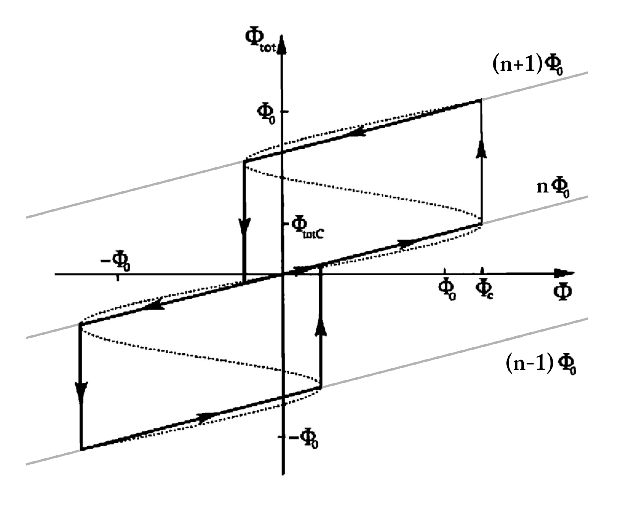
\includegraphics[width=0.9\linewidth]{pictures/squid_feld_verlauf.eps}
\caption{Verhalten des Flusses im SQUID bei Variation des äusseren Feldes.}
\end{figure}

In dem treibenden Schwingkreis (tank circuit) fliesst ein Strom $I_{rf}$ der einen Fluss $\Phi_{rf}$ erzeugt. Q ist hierbei der Qualitätsfaktor, der Übertragungsverluste berücksichtigt und M die Kopplung zwischen treibender Spule und Supraleiter.
\begin{align}
 \Phi_{rf}=MQI_{rf}
\end{align}




\subsection{Arbeitspunkt des SQUIDs}
Die Amplitude des Stromes im Schwingkreis wird sehr klein gewählt wird, so klein, dass die damit verbundene Flussänderung gegenüber dem Flussquant 
$\Phi_0$ verschwindend gering ist. Hierbei wird gebrauch davon gemacht, dass bei konstanter Stomapmplitude die Amplitude der Spannung im Schwingkreis abhängig vom anliegenden äußeren Feld variiert. Dies bedeutet, dass $V_{rf}$ dem Strom $I_{rf}$ folgt, solange der externe Fluss
nicht größer als der kritische Fluss ist (linearer Bereich). Bei kleinerem externen Fluss als ein Flussquant aber größer
als der kritische Fluss ergibt sich keine Änderung von $V_{rf}$ (Plateau). 

\begin{itemize}
 \item Falls $\Phi_{ext} = n \Phi_0$ , so entspricht die Amplitude der Spannung der Höhe des ersten Plateaus.
 \item Für ansteigendes $\Phi_{ext}$ wird der Hub der Spannung geringer, da das Plateau schon früher einsetzt.
       Das Minimum des Hubes wird erreicht, sofern der externe Fluss $\Phi_{ext} = (n + 1/2) \Phi_0$.
 \item Falls das externe Feld weiter anwächst, so steigt auch die Amplitude der Spannung, da der Strom eine Amplitude besitzt, welche bereits
       wieder über das Ende des Plateaus hinausgeht.
 \item Bei $\Phi_{ext} = (n + 1) \Phi_0$ wird schließlich das Maximum wieder erreicht.
\end{itemize}

Steigt der externe Fluss gleichmäßig an, so ändert sich die maximale Spannung im Schwingkreis periodisch. Die Periodendauer ist gekoppelt mit einer Änderung des externen Flusses um ganze Flussquanten $\Phi_0$.



\subsection{Lock-In Verstärker}
Bei der Methode des Lock-In Verstärkers wird dem zu messenden Signal ein Referenzsignal bekammter frequenz aufmoduliert.
Das somit erhaltene Signal und das Referenzsignal werden um 90Grad phasenverschoben auf einen Integrator gegeben. Hierbei wird die Orthogonalität von
sinus und cosinus ausgenutzt. Durch den Integrator werden somit alle Frequenzen die nicht dem Referenzsignal entsprechen, und somit jegliches Rauschen, herausgefiltert. \\

Wichtig ist das die Phasenverschiebung genau 90Grad beträgt. Im SQUID-Versuch ist dies durch die Elektronik fest eingestellt und muss daher vom Praktikanten nicht beachtet werden. Die einzige Einstellung die vorgenommen werden kann ist die größe des Kondensators im Integrator welche die Integrationszeit bestimmt und somit die Glättung des Signals beeinflusst.


\section{Versuchsaufbau}
Die Komponenten des SQUID-Versuchs:
\begin{itemize}
 \item Isoliertes Gefäß zur Aufnahme von flüssigem Stickstoff (Kryostat)
 \item Probenschlitten inklusive Aufsatz für zwei verschiedene Probenhalterungen - eine stromdurchflossene Leiterschleife und eine Mehrzweckhalterung
 \item Motor samt Spannungsversorgung und auf verschiedene Umdrehungsgeschwindigkeiten einstellbares Getriebe
 \item JSQ-Magnetometer, bestehend aus der SQUID-Sonde, deren Signalverarbeitungselektronik und Spannungsversorgung
 \item Oszilloskop zur Darstellung des SQUID-Signals
 \item Computer zur Auslese des Oszilloskopes und Steuerung des Regelkreises des SQUIDs
 \item Widerstände zwischen 50 Ω und 1000 Ω, sowie diverse Proben mit unbekanntem Dipolmoment
\end{itemize}

\subsection{JSQ-Magnetometer}
Das SQUID lässt sich uber die Software ’JSQ Duo Sensor Control’ bedienen. Hier lässt sich folgendes einstellen:
\begin{itemize}
 \item \textbf{VCA} - Die Stromamplitude des Schwingkreises. Die komplette Skala deckt, nicht ganz linear, einen
       Bereich von $-115~dBm ~(1, 8 ⋅ 10^{-9} W)$ bei einem eingestellten Wert von $0$ bis $-75~ dBm ~(1,8 ⋅ 10^{-7} W)$ bei einem Wert von $4095$.
 \item \textbf{VCO} - Regelung der Frequenz des Schwingkreises. Es können Werte von $630~MHz~(0)$ bis $970~MHz~(4095)$ eingestellt werden. Eine genaue
       Zuordnung findet sich im Benutzerhandbuch auf Seite 9.
 \item \textbf{OFF} - Dient zur Skalierung der Gesamtspannungsamplitude, dies wird hier dazu verwendet, das Signal um den Nullpunkt herum zu zentrieren.
 \item \textbf{Integr.C} - Kapazität des des Kondensators, welcher die Shaping-Zeit bestimmt. Größere Werte glätten das Signal mehr als kleine.
 \item \textbf{FB-R} Widerstandswert des sogenannten Feedback-Resistors. Durch seinen Wert wird die Spannung des Stromkreises festgelegt, was in
       diesem Fall die Verstärkung der Schaltung definiert. Je nach Einstellung gelten unterschiedliche Verhältnisse für die Relation von Spannung
       zur Anzahl der Flussquanten. Es sind folgende Werte des Transfer-Koeffizienten $s_i$ wählbar (Siehe auch Benutzerhandbuch Seite 25):
       \begin{center}
\begin{tabular}{lllllllll}
$R / k\Omega$ & 1 & 3 & 6 & 10 & 15 & 20 & 50 & 100\\
$s_i / mV / \Phi_0$ & 21 & 60 & 120 & 195 & 290 & 380 & 950 & 1900
       \end{tabular}
       \end{center}


\end{itemize}



\section{Durchführung}

\section{Auswertung}

\section{Zusammenfassung}



\end{document}
